\chapter{Tests and Results}

\paragraph{}
The Question Answer System implemented is part of the Yioop search engine and is platform independent. The system works by tagging phrases using a Brill variant Part of Speech tagger for Hindi sentences. In the next step, triplets are formed and stored in the database using the grammar rules for Hindi. The test data for the system is an index created by configuring Yioop to crawl hindi webpages from Wikipedia and Indian websites with Hindi content. We created 3 crawls about 100,000 webpages from which the summarizer extracted text from 6000 documents to create the index. Below are examples, of some 'Wh' questions to the system.

\section {Standalone Testcase}
In this section, we provide a text case for the system as standalone module. It is assumed that the input to the system is a semantically and syntactically correct sentence.

\begin{enumerate}
\item  Figure 9 shows the sentence after it is tagged for parts of speech

\begin{figure}[htb]
\centering
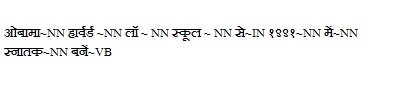
\includegraphics[width=0.8\textwidth]{images/sentence_testcase1.jpg}
\caption{Standalone Sentence 1.} 
\label{fig:sentence_testcase1}
\end{figure}

A word for word translation of the above sentence to English is 'Obama Harward law school from 1999 graduate complete'. From the translation, we can guess which words should go into the noun, post and verb phrases. Figure 10 shows the Parse Tree generated for this sentence 

\begin{figure}[htb]
\centering
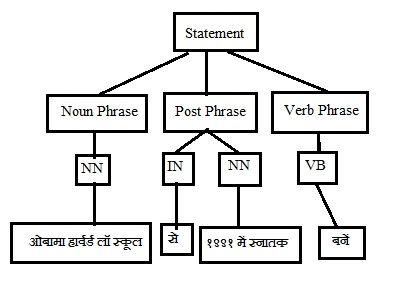
\includegraphics[width=0.8\textwidth]{images/standalone_testcase.jpg}
\caption{Parse Tree for sentence in Figure 9.} 
\label{fig:standalone_testcase}
\end{figure}

\paragraph{}
The triplets extracted for the above parse tree are as shown in Figure 11 above.

\begin{figure}[htb]
\centering
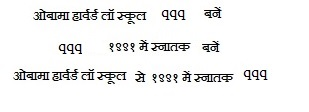
\includegraphics[width=0.8\textwidth]{images/triplet_standalone.jpg}
\caption{Triplets Extracted for sentence Figure 9.} 
\label{fig:triplet_standalone}
\end{figure}

\break
\item  Figure 12 shows the sentence after it is tagged for parts of speech

\begin{figure}[htb]
\centering
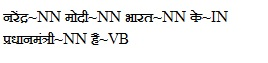
\includegraphics[width=0.5\textwidth]{images/sentence_testcase2.jpg}
\caption{Standalone Sentence 2.} 
\label{fig:sentence_testcase2}
\end{figure}

A word for word translation of the above sentence to English is 'Narendra Modi India (s) Prime Minister is'. From the translation, we can guess which words should go into the noun, post and verb phrases. Figure 13 shows the Parse Tree generated for this sentence 

\begin{figure}[htb]
\centering
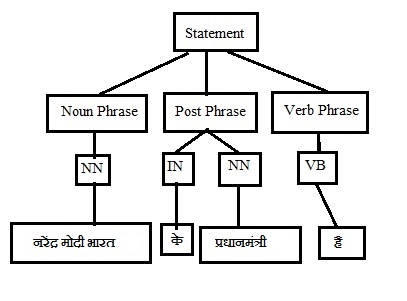
\includegraphics[width=0.8\textwidth]{images/standalone_testcase2.jpg}
\caption{Parse Tree for sentence in Figure 12.} 
\label{fig:standalone_testcase2}
\end{figure}

\end{enumerate}

\break
\section{Question Answer Module Integrated in Yioop}
\paragraph{}
Below are results for the Question Answer System when a crawl was setup for all wikipedia pages in Hindi, Indian websites. We set up a crawl by configuring Yioop in under crawl options. For the crawl, we restrict the crawler to websites from domains 'hi.wikipedia.org', 'co.in' and 'in'. We stopped the crawl was after we hit 200,000 webpages. The crawler extracted information from 7925 webpages to create the index. Figure 14, Figure 15, Figure 16 show the results after the Question Answer system is integrated in Yioop. 

\begin{figure}[htb]
\centering
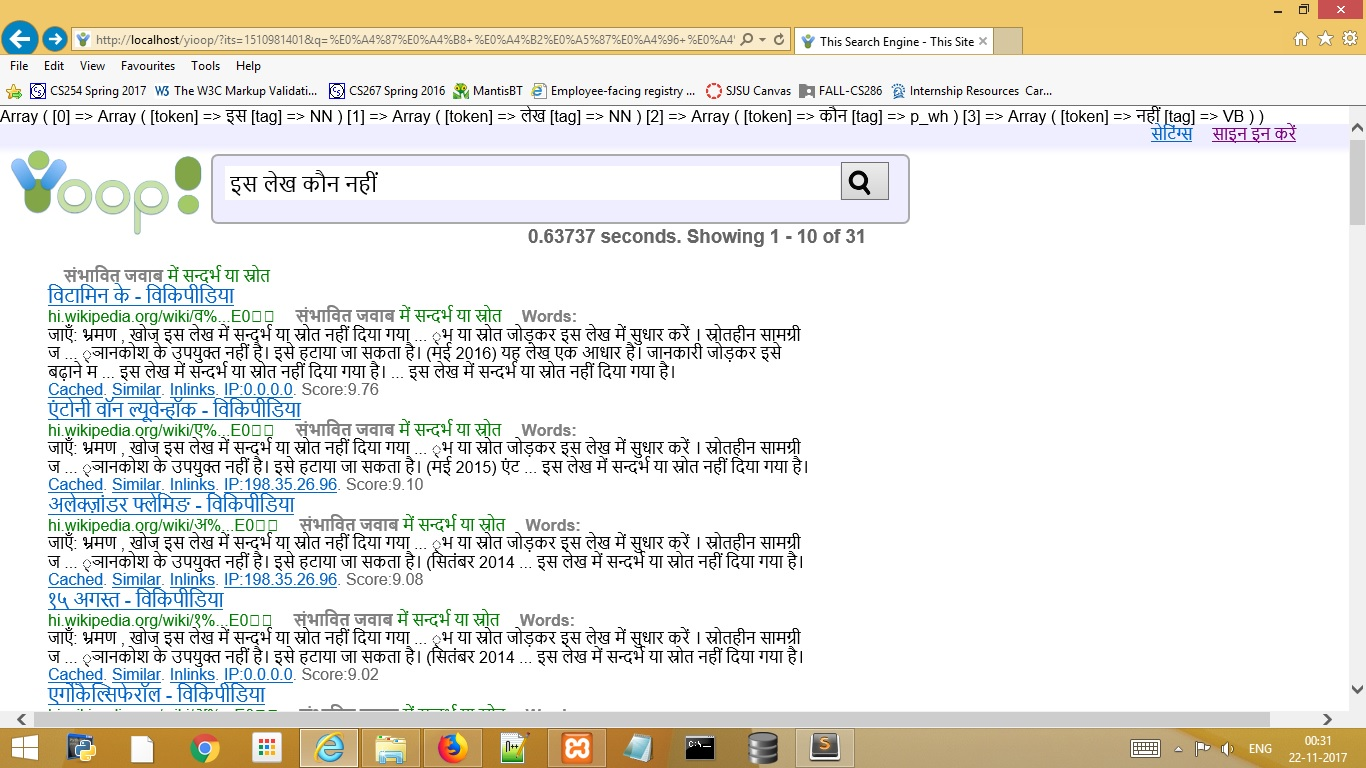
\includegraphics[width=0.8\textwidth]{images/who_question.jpg}
\caption{Who question after Integration in Yioop.} 
\label{fig:who_question}
\end{figure}
\break

\begin{figure}[htb]
\centering
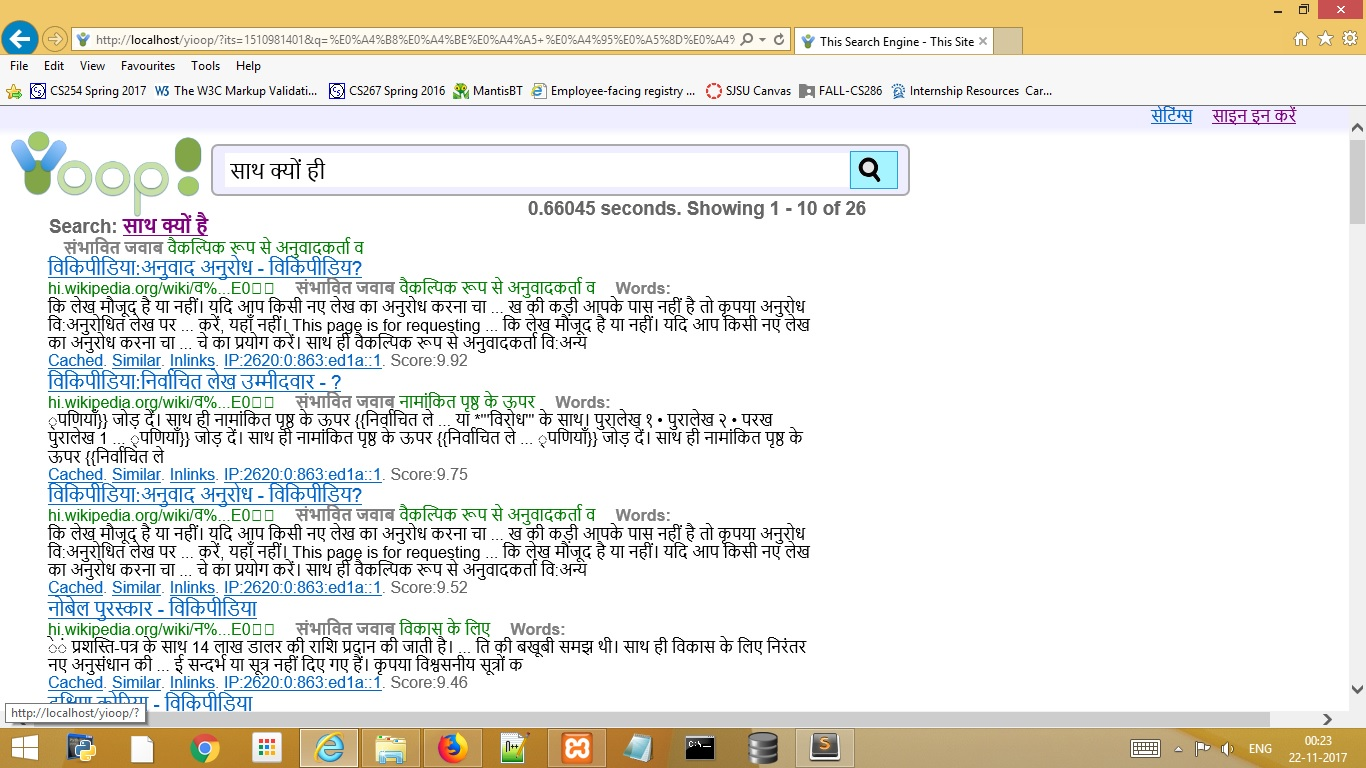
\includegraphics[width=0.8\textwidth]{images/why_question.jpg}
\caption{Why Question after Integration in Yioop.} 
\label{fig:why_question}
\end{figure}

\begin{figure}[htb]
\centering
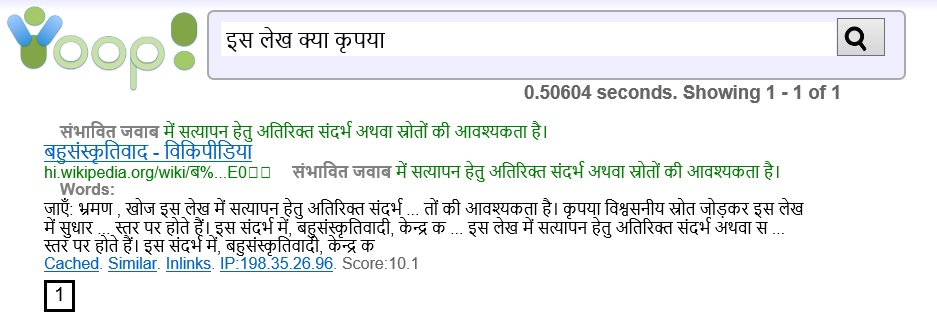
\includegraphics[width=0.8\textwidth]{images/what_question.jpg}
\caption{What Question after Integration in Yioop.} 
\label{fig:what_question}
\end{figure}

\paragraph{}
The integration of the Question Answer system slows down Yioop as extra processing is performed for generating and storing the triplets. But the performance improves for query time as whenever user enters a question it is looked up directly from a map. Figure 17 shows the time impact when we asked a simple question in Hindi.

\begin{figure}[htb]
\centering
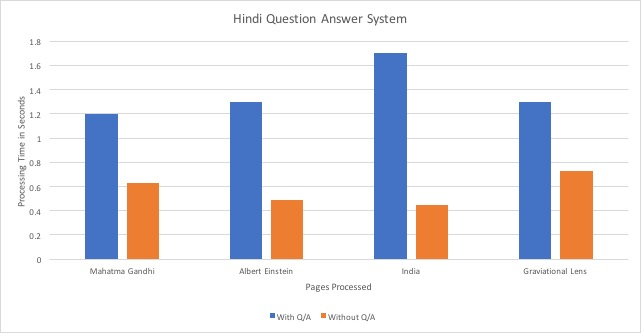
\includegraphics[width=0.8\textwidth]{images/QA_performance1.jpg}
\caption{Yioop performance for simple Hindi Questions.} 
\label{fig:QA_performance1}
\end{figure}

\paragraph{}
The initial implementation of the Question Answer system read performed part of speech tagging by reading a file based lexicon from a file. It performed a sequential search on the lexicon read in memory, Figure 18 shows the improvement in part of speech tagging, as words are tagged from the database indexed on term and locale. For the test, I used 1000 - 1500 word paragraphs for each of the subjects as input to the two variants of the part of speech tagger module.

\begin{figure}[htb]
\centering
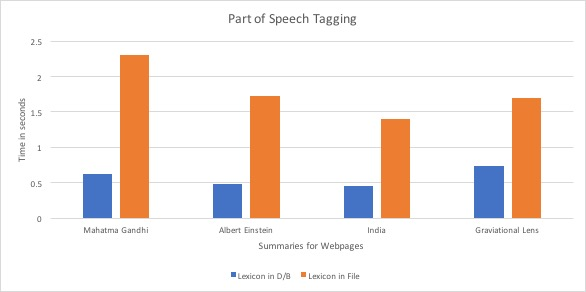
\includegraphics[width=0.8\textwidth]{images/QA_performance2.jpg}
\caption{Yioop performance for simple Hindi Questions.} 
\label{fig:QA_performance2}
\end{figure}
\break

\paragraph{}
We compare the English and Hindi Question answer systems for relevant answers. I used 4 subjects on which I asked the same question in English and Hindi. Figure 19 shows the number of relevant answers returned on Page 1 of search result. We can see that English system is better at providing more accurate answers compared to Hindi.

\begin{figure}[htb]
\centering
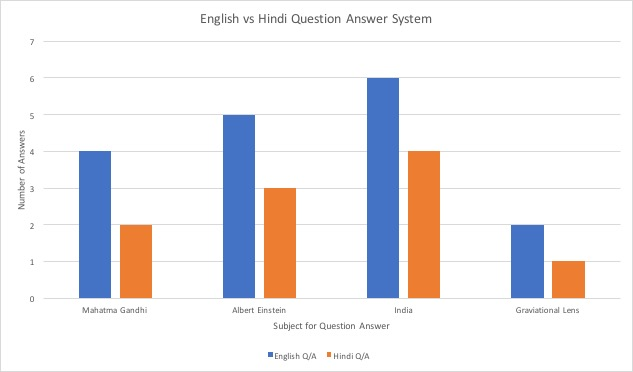
\includegraphics[width=0.8\textwidth]{images/QA_performance3.jpg}
\caption{Yioop performance for simple Hindi Questions.} 
\label{fig:QA_performance3}
\end{figure}